\section{Tuning Methodology } %3.4
\label{section3.4}
\subsection{Tuning Model} %3.4.1
Imagine if we have a 2D plane with the horizontal axis kp and the vertical axis ki, we can use the points on the plane to represent all the acceptable combination of kp and ki.\\

\begin{figure}[!htbp]
\minipage{0.33\textwidth}
  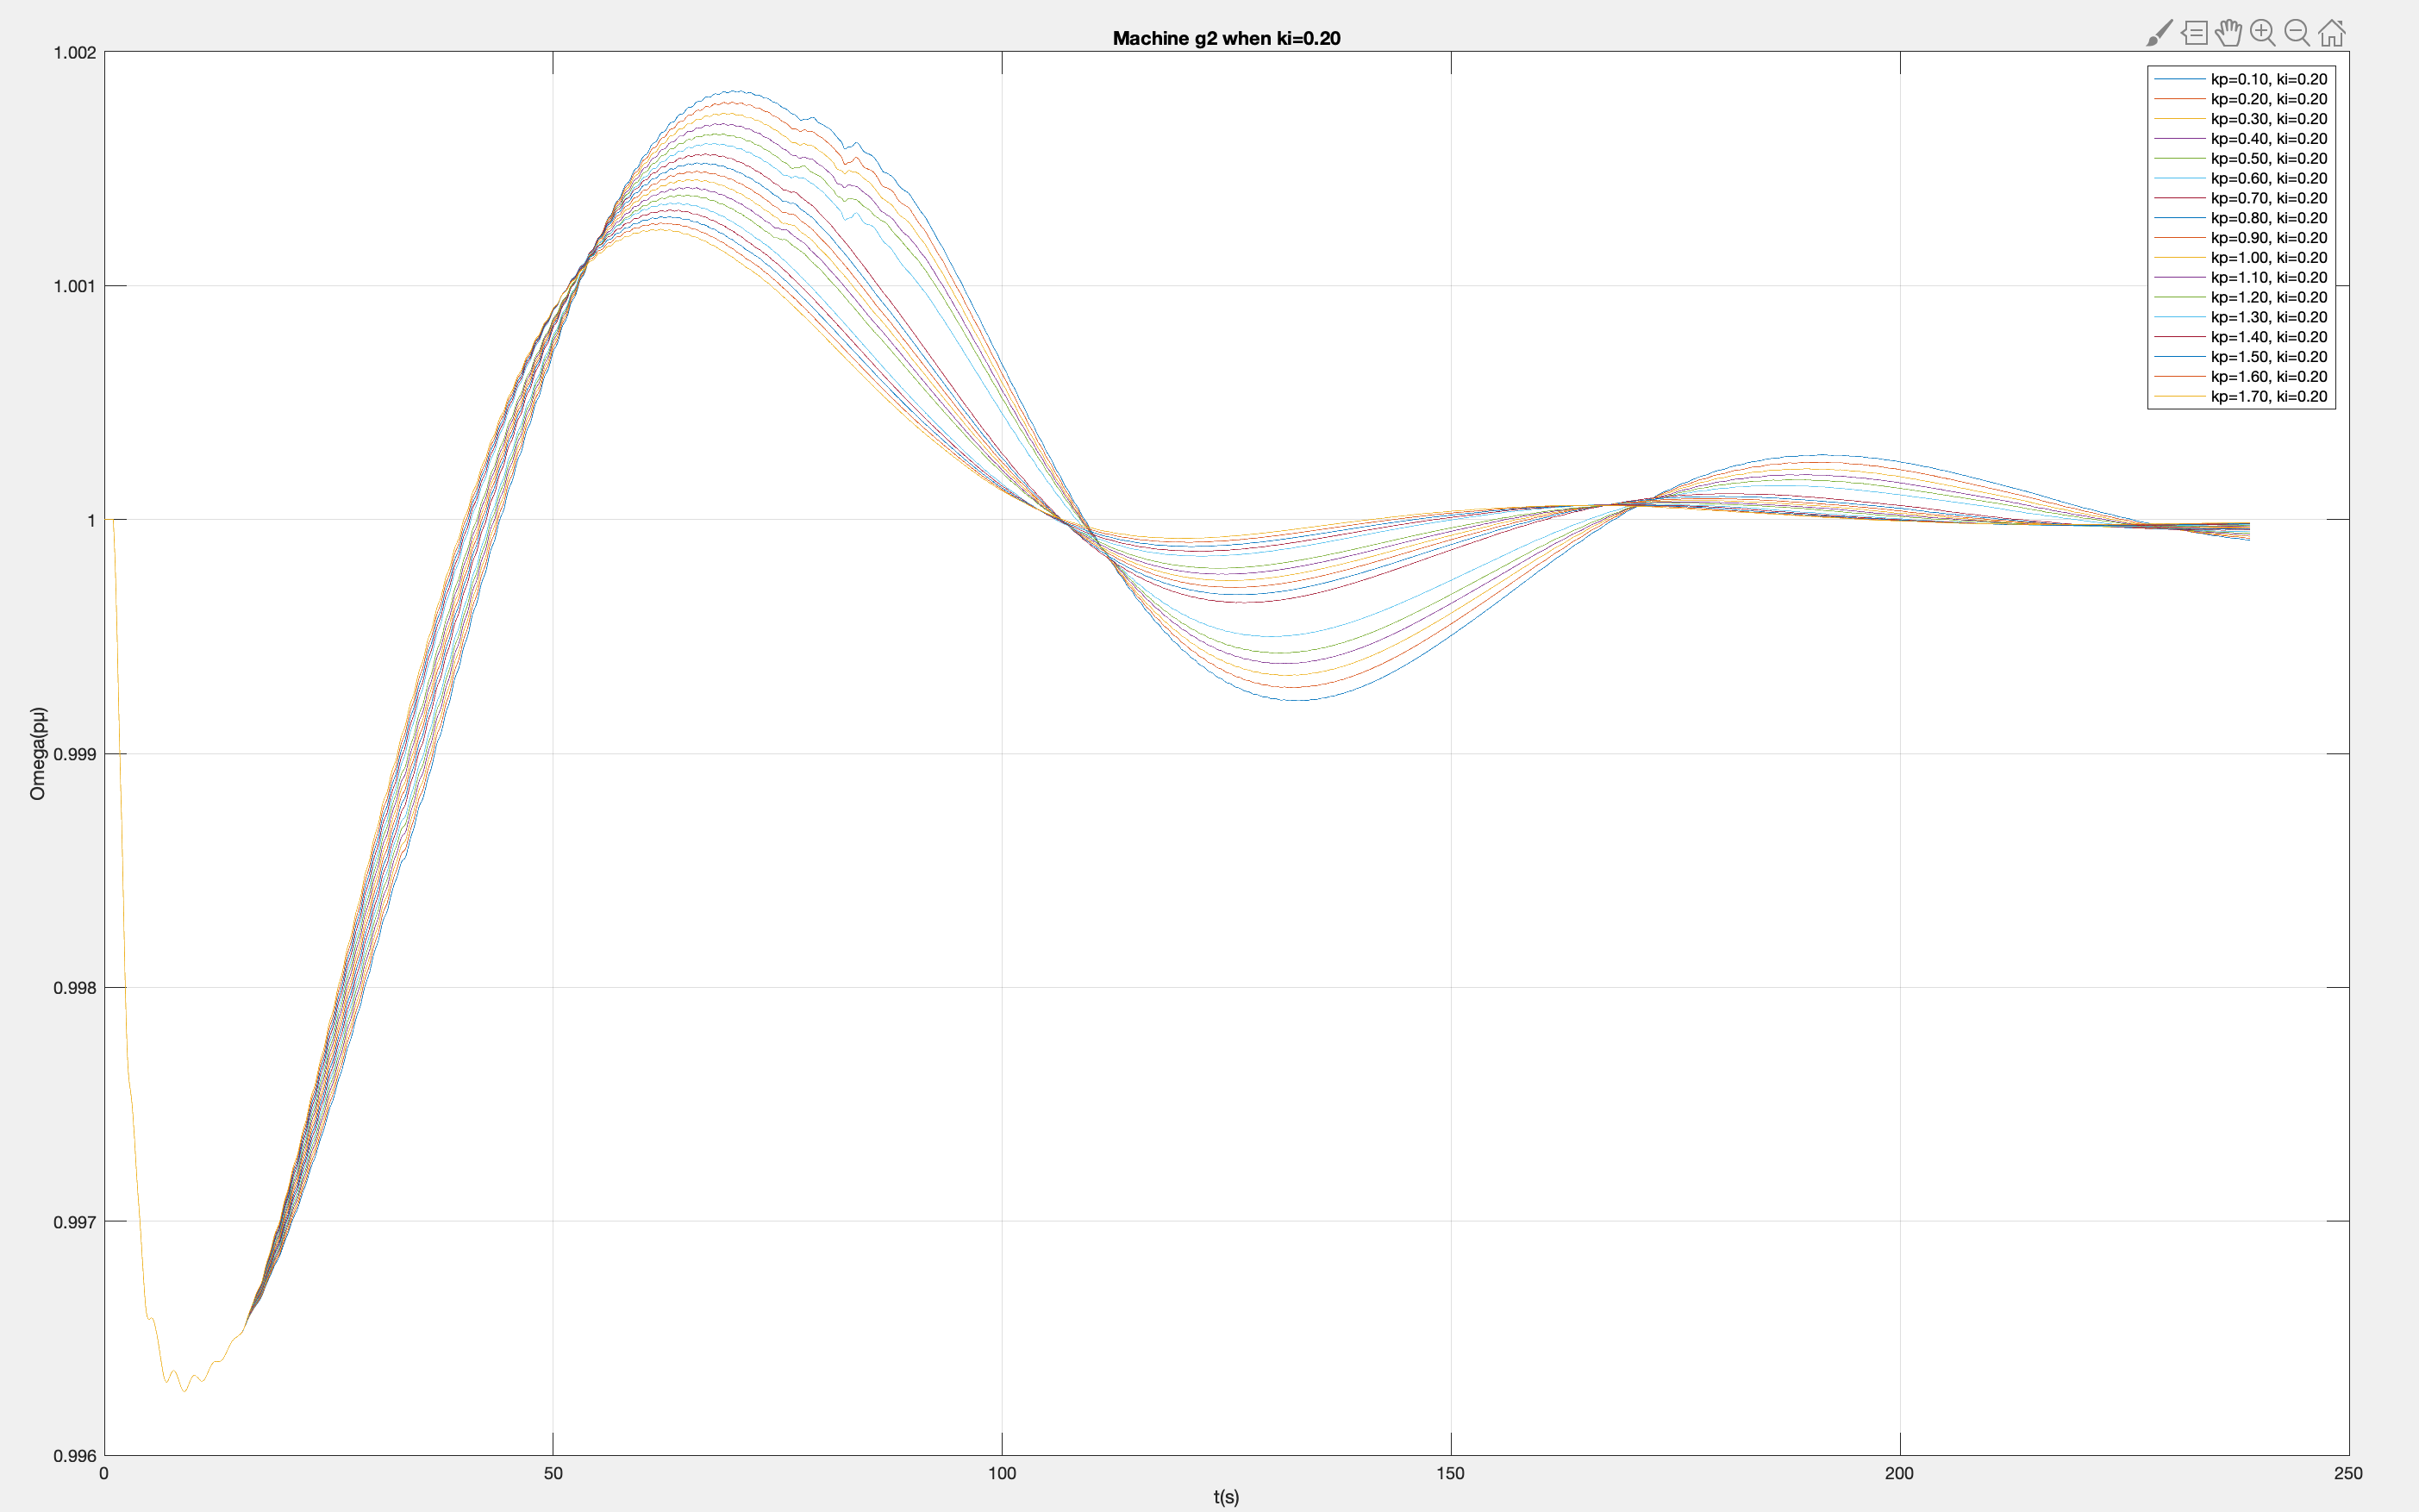
\includegraphics[width= \linewidth]{figure/3_4_1_tune_ki_1.png}
  %\caption{A really Awesome Image}\label{fig:awesome_image1}
\endminipage\hfill
\minipage{0.33\textwidth}
  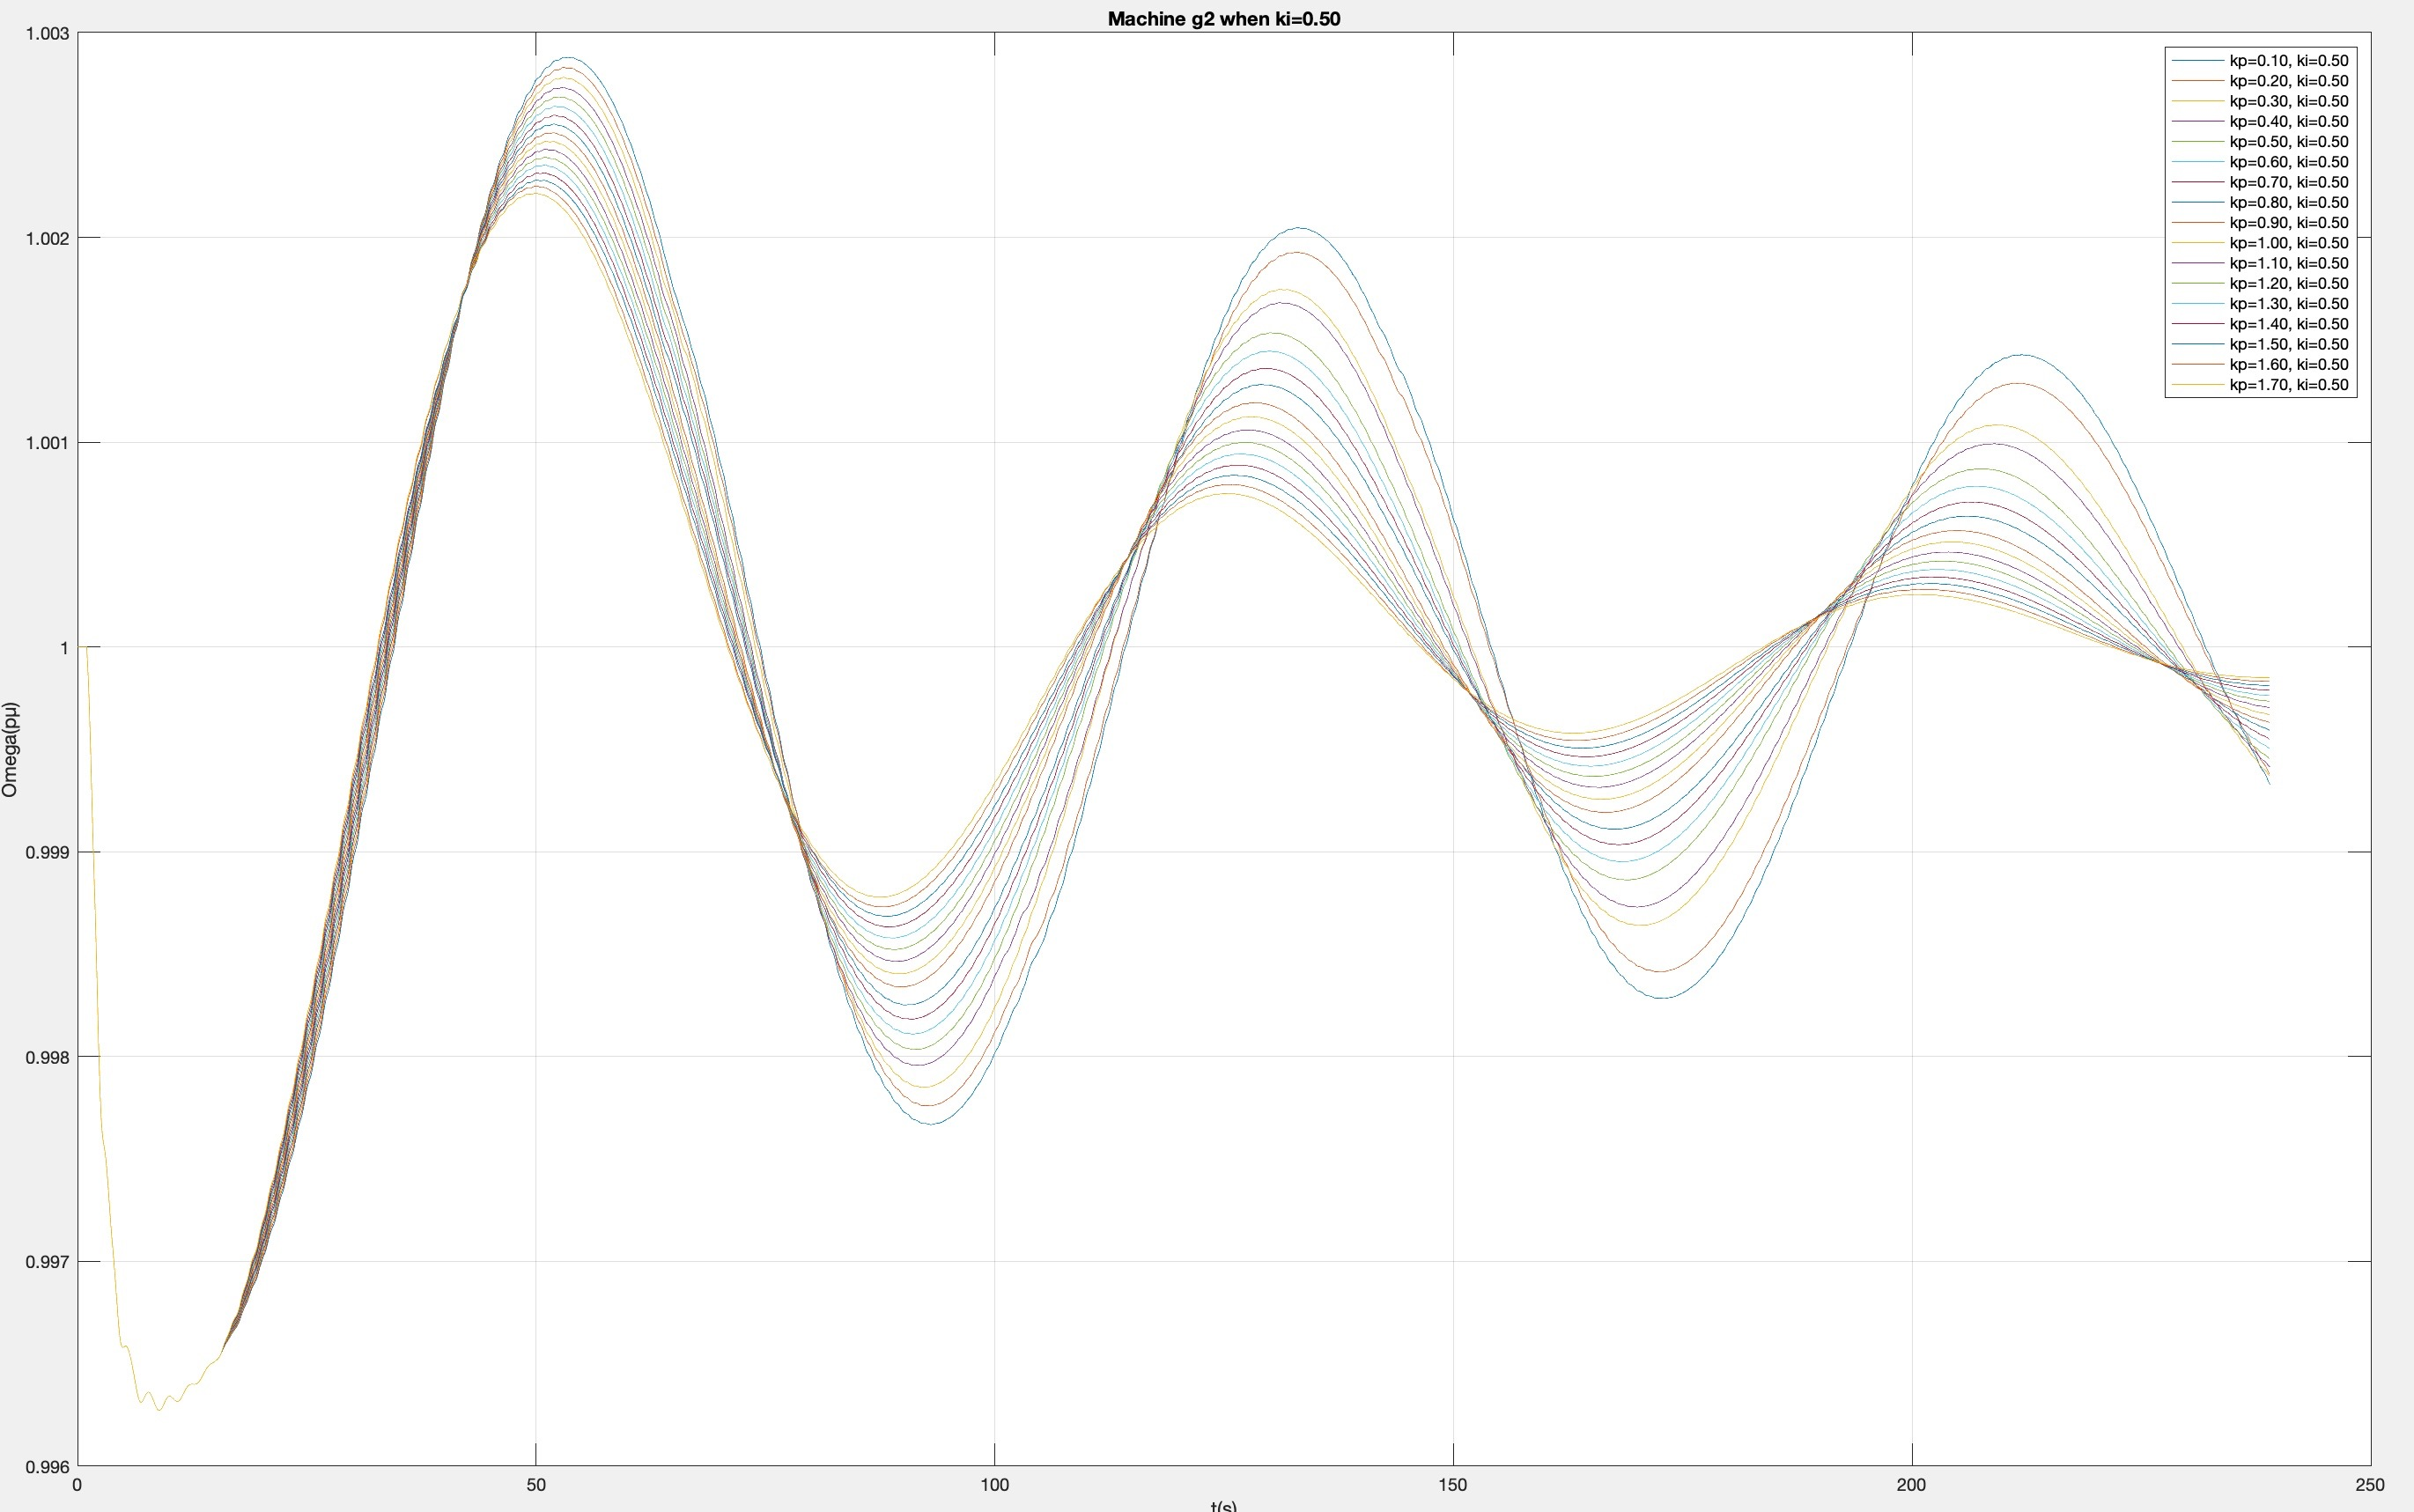
\includegraphics[width= \linewidth]{figure/3_4_1_tune_ki_2.jpeg}
  %\caption{A really Awesome Image}\label{fig:awesome_image2}
\endminipage\hfill
\minipage{0.33\textwidth}%
  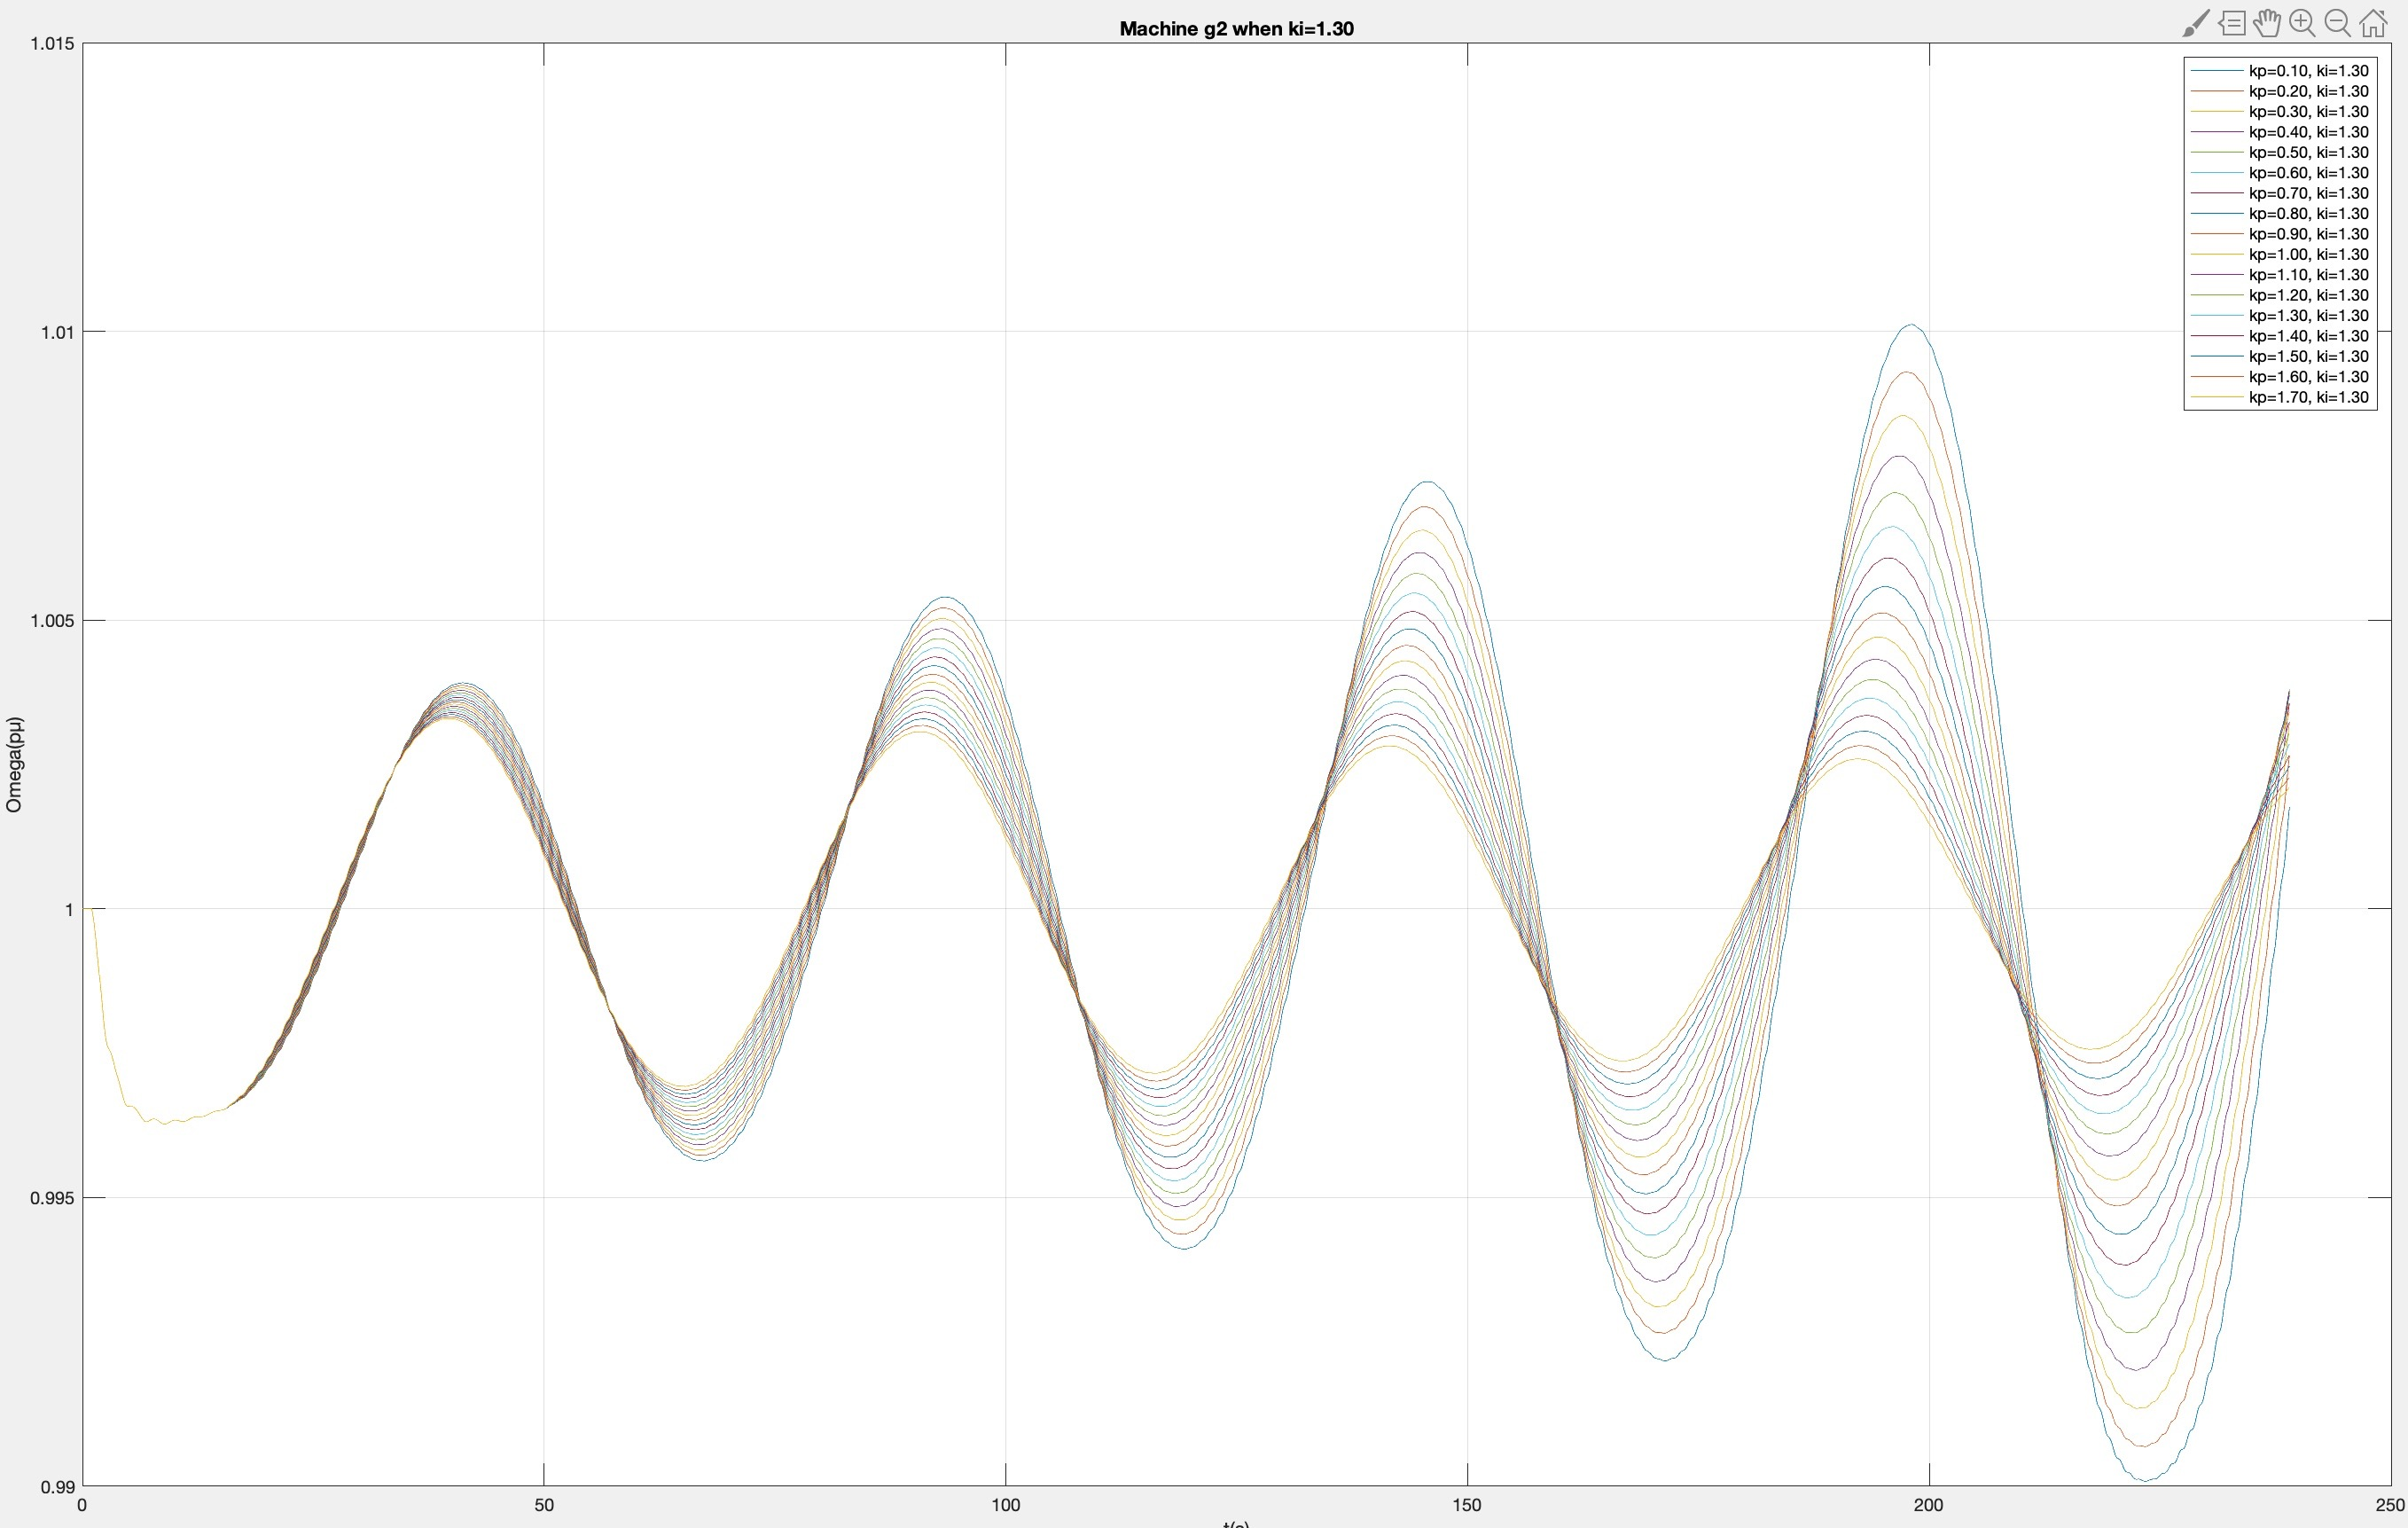
\includegraphics[width= \linewidth]{figure/3_4_1_tune_ki_3.jpeg}
  %\caption{A really Awesome Image}\label{fig:awesome_image3}
\endminipage
\caption{PI Control: ki = 0.2; ki = 0.5; ki = 1.3.}
\label{3_4_1_larger_ki}
\end{figure}


The reason for this is that neither kp nor ki can be infinitely magnified. Kp is the amplifier factor of D-term and it represents how quickly an error can be corrected. If kp is larger, the overshoot of the corrected signal will be larger. Kp has a limit because there is an acceptable range of frequency with official document. For instance, in Nordic test case scenario, the limit is ±0.2\%. In other words, the range of signal is from 0.998 $p\mu$ to 1.002$p\mu$.\\

Ki is the amplifier factor of the I-term. The signal have too many oscillations and it not be settled if we keep increasing the value of ki. 
However, the signal needs to be settled before a specific time in reality and it makes sure the signal be no chance of excessive oscillation. Thus, ki is limited.\\

One of the objectives of this project is to find the best combination of amplifier factors, i.e. kp and ki. To obtain it, we need to find the limit of kp and ki and simulate possible situations in the range.\\

The idea of bisection method is used to find the limit of kp and ki.\\

Firstly, we tune a large kp, and we test if a new signal is acceptable. To simplify the model, we choose ki being from 0.1 to the value of kp and the step of ki is dependent to the value of kp. For instance, if kp is 500.1, the range of ki is between 0.1 and 500.1. From the part we discussed before, the signal has great chance to have a large overshoot. Thus, ki can be given a large step, like 100.0. We do not need to worry about such a large step will filter some acceptable results. The purpose of this step is not to find all the acceptable results. The purpose of tuning kp and ki is not finding all the possible values. We hope to find a general relationship between kp and ki and it will be helpful to find the impact of time delay afterwards.\\

Secondly, we check if the signal is acceptable if we have simulated data. The purpose of this step is to find the limit of ki.\\

If ki exists (i.e. there is one acceptable result at least), for instance, ki equals to 200.1, we need to make sure there be no solutions when increasing ki by its step. Then, we can judge that the limit of the kp is between (200.1 and 200.1 + the step of kp). Thus, we have a range of kp which is between (0.1 and 200.1 + the step of kp). If the step of kp is 10, the range of kp will be from 0.1 to 210.1. Normally, we can directly tune kp and ki between 0.1 and 210.1.\\

If ki exists in another way, for instance, kp equals to 200.1 and ki equals to 5.1 when the step of ki is 5.0. The result is acceptable but we need to increase the value of kp to make sure ki not exist when kp equals to (kp + the step of kp).\\

If ki does not exist, for instance, there is no acceptable ki when kp is 500.1. According to bisection method, we can test the simulations and tune kp between 0.1 and 250.1. We repeat the method above until we find the limit of kp and ki.\\


\subsection{Analytical Models} %3.4.2
\label{subsection3.4.2}
The first analytical model generates two different kinds of excel files. One of them is named as ori.xlsx. This is a file saving all the acceptable results. For another kind of files, their names are related to the value of time delay. For instance, if time delay is 0.01 seconds, the file name be td\_0.01s\_xlsx. It store all the acceptable results when delay is 0.01 seconds.\\

Importantly, we define 'SettlingTimeThreshold' , a MATLAB variant, to 0.02, so the time take for the error between the response and the steady-state response to fall to within 2\% of nominal value.\\

\begin{figure}[htbp]
\centering
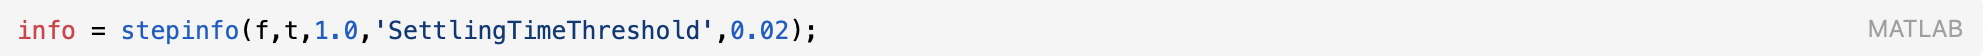
\includegraphics[width = .999\textwidth]{figure/3_4_2_code4.png}
\caption{MATLAB: stepinfo function.}
\label{3_4_2_code4}
\end{figure}

In our case, the system start from 0 second. However, in the analytical model, we can not put all the data into the stepinfo function because we do not want the data without SFC be calculated. Thus, the data stepinfo function gets should starts from the SFC control starting, which is the 150th seconds. \\

\begin{figure}[htbp]
\centering
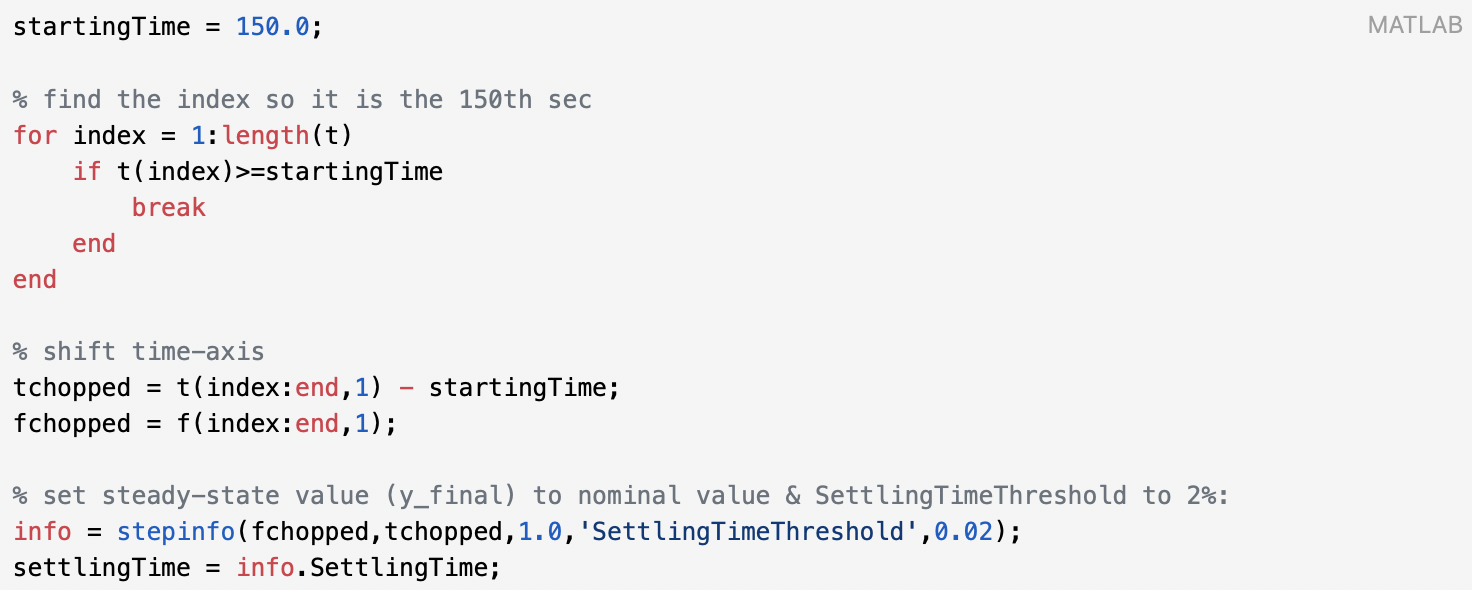
\includegraphics[width = .999\textwidth]{figure/3_4_2_chopped.png}
\caption{MATLAB: chopped the time from the 150th sec.}
\label{3_4_2_chopped}
\end{figure}


In the first analytical model named i\_cur\_plot.cur , we check if simulation results are acceptable via our MATLAB program if we have collected data. Firstly, we import data from simulations. Then, we limit both the overshoot and settling time as required via a MATLAB module: stepinfo. The data will be filtered if the overshoot or the settling time is not in the required range.\\

\begin{figure}[htbp]
\centering
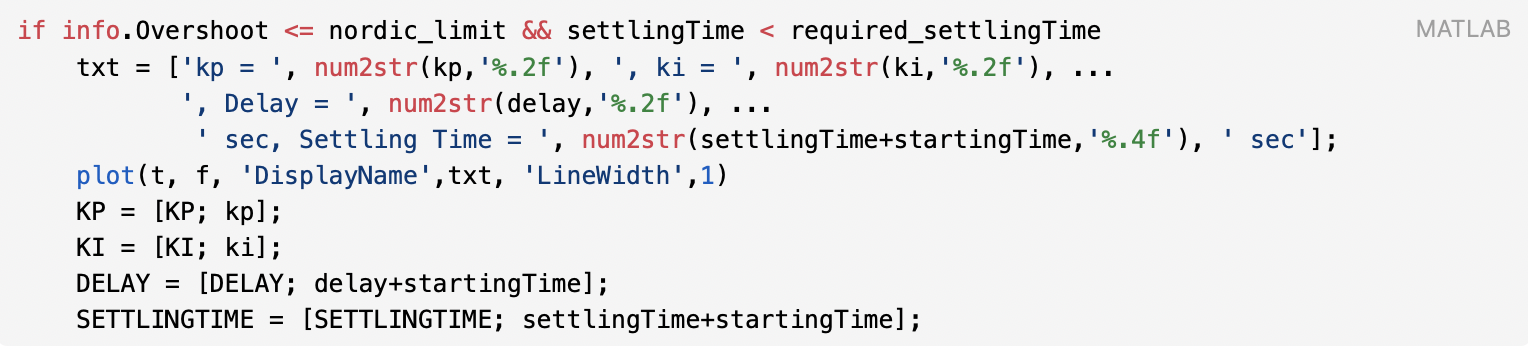
\includegraphics[width = .999\textwidth]{figure/3_4_2_code5.png}
\caption{MATLAB: filter unacceptable tuning results.}
\label{3_4_2_code5}
\end{figure}


As you can see from Figure~\ref{3_4_2_code5}, if the signal is acceptable, its parameters, i.e. kp, ki and time delay, will be saved in prepared lists. The lists will be transferred into the two kinds of excel files.\\

The second analytical model helps finding which combination of kp and ki has a minimum settling time with a fixed delay. The idea is as follows. Firstly, we import an excel file, whose name is related to the value of delay,  that is generated by the last step. Then, we find the minimum settling time. Finally, we find related kp, ki and delay and export them into another excel file.\\

The third analytical model helps finding the best combination of kp and ki. Firstly, we import data from ori.csv. Then, we calculate the average settling time for each combination of kp and ki. However, it is invalid that a combination is not acceptable for all the time delay. Thus, we need to add a limitation factor to make sure the best combination is valid for every delay. For instance, if there are 21 different time delays, we can use\\

\begin{figure}[htbp]
\centering
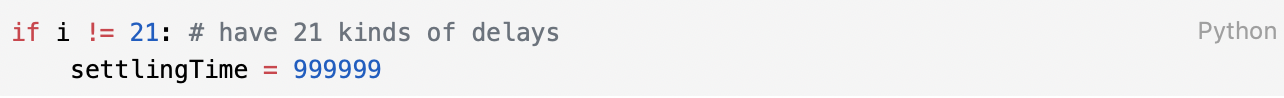
\includegraphics[width = .999\textwidth]{figure/3_4_2_code6.png}
\caption{Python: filter out the tuning results that cannot settled in all delay}
\label{3_4_2_code6}
\end{figure}

to filter some unacceptable results. Finally, we have all the average settling tim so we can find the minimum average settling time.\\

The fourth analytical model helps sorting out the combination’s settling time with different time delay. It is one of the inputs of the fifth analytical model.\\

The fifth analytical model helps plotting a 3D triangle surface diagram. It draws a 3d plot from the data in ori.xlsx. We use:\\

\begin{figure}[htbp]
\centering
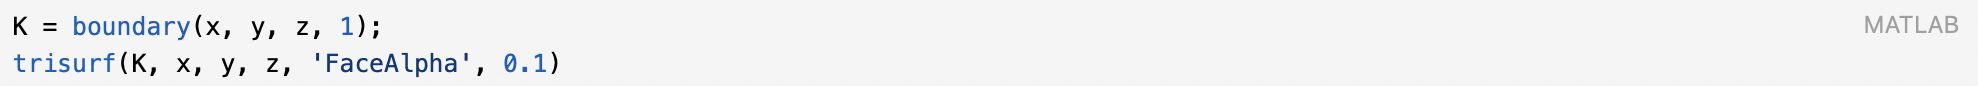
\includegraphics[width = .999\textwidth]{figure/3_4_2_code7.png}
\caption{MATLAB: 3D triangle surface algorithm.}
\label{3_4_2_code7}
\end{figure}

to draw a triangle surface plot. Besides, it highlights the results from the second analytical model and the fourth analytical model. With a 3D triangle surface plot, we can clearly understand the impacts of the time delay.\\